\chapter{What is computer software?}

\begin{figure}
    \centering
    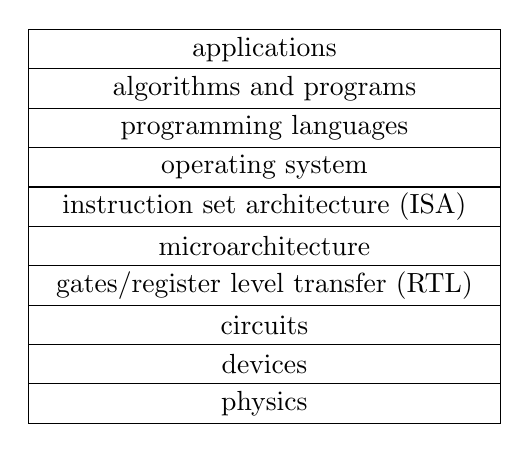
\begin{tikzpicture}
        \draw (0,0) rectangle node{physics} (6,0.5);
        \draw (0,0.5) rectangle node{devices} (6,1);
        \draw (0,1) rectangle node{circuits} (6,1.5);
        \draw (0,1.5) rectangle node{gates/register level transfer (RTL)} (6,2);
        \draw (0,2) rectangle node{microarchitecture} (6,2.5);
        \draw (0,2.5) rectangle node{instruction set architecture (ISA)} (6,3);
        \draw (0,3) rectangle node{operating system} (6,3.5);
        \draw (0,3.5) rectangle node{programming languages} (6,4);
        \draw (0,4) rectangle node{algorithms and programs} (6,4.5);
        \draw (0,4.5) rectangle node{applications} (6,5);
    \end{tikzpicture}
    \caption{Layers of abstraction in a modern computer system.}
\end{figure}

\section{Algorithms and programming languages}

\begin{definition}
    An \textbf{algorithm} is a method or a process followed to solve a problem. An algorithm must meet the following criteria:
    \begin{enumerate}
        \item correctness, that is, it solves the problem it is designed for;
        \item composed of concrete unambiguous steps;
        \item the number of steps must be finite; and
        \item must terminate.
    \end{enumerate}
\end{definition}

\begin{definition}[Programming language]
    A \textbf{programming language} provides a means for translating an a \textbf{algorithm} into a form suitable for execution by a computer.
\end{definition}

An algorithm is \emph{not} a computer program. A program is written in a strict, explicitly defined programming language. An algorithm may have many different implementations.

\section{Programming languages}

\begin{definition}[Programming paradigm]
    \textbf{Programming paradigms} are just a way of classifying different programming languages based on features, a language can have more than one paradigm.
\end{definition}


\begin{example}[Programming paradigms]
    Some programming paradigms include:
    \begin{enumerate}
        \item imperative, statements change a program's \textbf{state} such as Python, C, \ldots;
        \item declarative, programs say what they want to do rather than \emph{how}:
        \begin{enumerate}
            \item functional, programs are defined as mathematical functions such as Haskell, Lisp, \ldots;
            \item logical, programs specify a logical solution;
        \end{enumerate}
        \item data-oriented, programs that work with data through manipulating and searching relations (tables) such as SQL, dBase, \ldots;
        \item scripting, designed to automate frequently used tasks that involve calling or passing commands to external programs (to \emph{glue} programs together) such as Python, Javascript, \ldots.
    \end{enumerate}
\end{example}

\begin{example}[More programming paradigms]
    \begin{enumerate}
        Other, less common programming paradigms include:
        \item assembly, a \emph{low-level} programming languages and that provides interface between machine code and a high-level programming language;
        \item concurrent, a language that provides facilities for concurrency (threads, processes) with featuers such as \textbf{message-passing} or \textbf{shared-memory};
        \item dataflow, a program specified by flow of data;
        \item fourth-generation, high-level languages built around databases;
        \item list-based, \ldots;
        \item visual, allow user to specify programs using visual representations.
    \end{enumerate}
\end{example}

There are hundreds of different languages all that fit into different groups of paradigms, this begs the question of why do we need so many languages? 

\begin{enumerate}
    \item \textbf{Productivity} Programming languages such as C and Java are very verbose and detailed which leads to many lines of code which leads to lots of expense in development and maintenance. 
    \item \textbf{Reliability} It is difficult to design computer programs that are correct. Some programming languages have features so that programs written in them will be nmore reliable, such as:
    \begin{enumerate}
        \item type checking, making sure operations that are forbidden between two types do not rise in execution (e.g. the expression $('a'>4)$ should not be compiled);
        \item exception handling, gives a program the ability to deal with errors that arise during execution.
    \end{enumerate}
    \item \textbf{Security} Some programming languages need to have layers of security such that we can use them without them being exploited maliciously. For example, a Javascript script can be downloaded and executed on your own machine when you visit the web-page, so the activities that can be done inside Javascript are limited.
    \item \textbf{Execution speed} As new technology is developed in Computer Science, we have to develop our programming languages to exploit the advances. For example, parallel computing calls for a new programming paradigm in which we split execution into multiple threads that can run on separate threads.
    \item \textbf{Curiosity} As new ideas about how things might be done differently emerge, so do programming language designers build new languages exploiting the concept.
    \item \textbf{Style} Individual programmers have varying preferences and styles for programming languages.
\end{enumerate}

When designing programming languages we should design them to be:

\begin{enumerate}
    \item be easy to use, with its program being easy to read, write, and understand;
    \item support \emph{abstraction} such that adding new features and concepts should be viable;
    \item support testing, debugging and program verification 
    \item inexpensive to use, in terms of execution time, memory usage, and maintenance costs.
\end{enumerate}

\section{Overview on logic programming}

\begin{definition}
    Logic programming is a programming paradigm that uses mathematical logic in order to computer.
\end{definition}

Logic programming can be used:

\begin{enumerate}
    \item procedurally, $A \implies B$; or
    \item declaratively $A = \text{True}$.
\end{enumerate}

Let's look at a few examples in Prolog.

\begin{example}[Prolog declarative statements]
    Take the following Prolog program.
    \begin{lstlisting}[language = Prolog]
female(artemis).
male(apollo).
parents(uranus, gaia, rhea).
parents(cronus, rhea, hera).
mother(gaia, uranus).
    \end{lstlisting}
    We can interpret these facts as follows:
    \begin{enumerate}
        \item \texttt{female(artemis).}, Artemis is female;
        \item \texttt{male(apollo).}, Apollo is male;
        \item \texttt{parents(uranus, gaia, rhea).}, Uranus and Gaia are parents of Rhea;
        \item \texttt{parents(cronus, rhea, hera).}, Cronus and Rhea are parents of Hera; and
        \item \texttt{mother(gaia, uranus).}, Gaia is the mother of Uranus.
    \end{enumerate}
\end{example}

\begin{example}[Prolog procedurral statements]
    Take the following Prolog program.
    \begin{lstlisting}[language = Prolog]
mother(X, Y) :- parents(_, X, Y).
female(X) :- mother(X, _).
sibling(X, Y) :- parents(_, _, X), parents(_, _, Y), X \= Y.
    \end{lstlisting}
    Note that \texttt{:-} is to be read as `is implied by'. So we can interprete the rules above as:
    \begin{enumerate}
        \item \texttt{mother(X, Y) :- parents(\_, X, Y).} if $X$ is the second parents of $Y$ then $X$ is the mother of $Y$;
        \item \texttt{female(X) :- mother(X, \_).} if $X$ is a mother she is female; and
        \item \texttt{sibling(X, Y) :- parents(A, B, X), parents(A, B, Y), X \textbackslash = Y.} if $X$ has parents $A$ and $B$, $Y$ has parents $A$ and $B$, and $X$ does not equal $Y$ then $X$ and $Y$ are siblings.
    \end{enumerate}
\end{example}

\section{Programming in parallel}

The following are reasons to program in parallel:

\begin{enumerate}
    \item \textbf{Performance}. Multi-core processor are common so we need to write parallel programs to improve performance.
    
    \item \textbf{Hiding latency}. Even on single core processor, we can exploit programs to hide latency of slow input and output operations to disk and network devices.
    
    \item \textbf{Software structuring}. Soem programs are naturally suited to a parallel programming paradigm. %Such as?
    
    \item \textbf{Real world concurrency}. Real world situations present requirements for concurrent programming, such as handling multiple server requests at once.
\end{enumerate}

\section{Ubiquitous/pervasive computing}

\begin{definition}
    \textbf{Ubiquitous} or \textbf{pervasive computing} is the integration of computers and software into everyday objects and activities.
\end{definition}

One enabling technology for ubiquitous computing is radio frequency identification (RFID) that uses radio waves to transfer data from an electronic tag to a reader. These can either be active (having their own energy source) or passive (where they operate using energy transmitted by the reader). 

Green computing is an evolving area of Computer Science which involves anything to do with energy conservatrion within information technology. This can range from designing chips which use less power to writing programs with the focus of reducing the energy expanded (such as putting devices to sleep when not needed).

\section{Syntax and semantics}

\begin{definition}
    The \textbf{syntax} of a programming language is how it is written.
\end{definition}

\begin{definition}
    The \textbf{semantics} of a programming is what it means.
\end{definition}

In Computer Science, informality in semantics will lead to ambiguity that will cause divergence which leads to errors. Computer Science uses Mathematics (set theory, logic, and category theory) to define different types of formal semantics:

\begin{enumerate}
    \item \textbf{denotational semantics}, a program's meaning is given mathematically as a suitable mathematical structure (e.g. a function);
    
    \item \textbf{operational semantics}, a program's meaning is given in terms of the steps of a computation the program makes when it runs (state changes); and
    
    \item \textbf{axiomatic semantics}, a program's meaning is given indirectly in terms of a collection of logical properties it satisfies and how these properties are maintained.
\end{enumerate}

As computers become ever more pervasive, we are requiring stricter formal semantics for programming languages applied to safety critical settings, such as nuclear power plants and medical devices.

\section{Compilation vs. interpretation}

\begin{definition}[High-level programming language]
    A \textbf{high-level programming language} is a programming language with a high abstraction from the details of the computer. They are designed for humans to understand and write. 
\end{definition}

Compilation and interpretation are both methods for translating high-level code into low-level code (something that a computer can \emph{understand} and execute).

\begin{definition}[Compiler]
    A \textbf{compiler} transforms high-level program code to machine code for the CPU to execute.
\end{definition}

\begin{example}[Compiled languages]
    \textbf{C}, \textbf{C++}, \textbf{C\#}, \textbf{Java}, \textbf{Haskell}, and \textbf{Fortran} are all compiled languages.
\end{example}

\begin{definition}[Interpreter]
    A \textbf{interpreter} translates one instruction (or a small collection of instructions) of the high-level program code at a time, as it is needed.
\end{definition}

\begin{example}[Interpreted languages]
    \textbf{Python}, \textbf{Ruby}, and \textbf{Javascript} are all interpreted.
\end{example}

There are trade-offs as to whether compilation or interpretation is preferable:

\begin{enumerate}
    \item compiled languages tend to run faster;
    \item compilers spends time analysing and optimisating code;
    \item compilation avoids run time errors;
    \item compiled programs can typically only run on the platform they are compiled for;
    \item interpreted programs tend to use memory better;
    \item interpreted programs facilitate development as they are free from compilation times; and
    \item interpreted programs can be executed on any platform that has the interpreter.
\end{enumerate}

Some programming languages, such as Java, have their programs compiled into what is called \textbf{bytecode}. This is a intermediate code that is fast to interpret and then translated by a Java Virtual Machine for the target processor.

\section{Compilation}

Within compilation, we can describe four fundamental stages:
\begin{enumerate}
    \item lexical analysis;
    \item syntax analysis; 
    \item translation phase; and
    \item code generation.
\end{enumerate}

\begin{definition}[Lexical analysis]
    We can think of the \textbf{lexical analyser} as a function $L$ that converts a sequence of characters into a sequence of \textbf{tokens} (basic syntactic components), more formally \[ L : C^n \to T^m \] where $C$ is the set of valid characters and $T$ is the set of all tokens.
\end{definition}

\begin{example}[Lexical analysis]
    As an illustration, consider the following piece of code.
    \begin{lstlisting}
{
    let x = 1;
    x := x + y;
}
    \end{lstlisting}
    This might be converted  to the following token stream.
    \begin{lstlisting}
LBRACE LET ID/x EQ NUM/1 SEMIC ID/x ASS ID/x PLUS ID/y SEMIC RBRACE
    \end{lstlisting}
    This is clearly harder to read than the original code, but it easier for the computer to process.
\end{example}

\begin{definition}[Syntax analysis (or parser)]
    The \textbf{syntax analyser} will start to recognise some structure to the code, it will form a \textbf{parse tree} from the token stream, as below. This tree is simplied and redundant information is taken out.
\end{definition}

\begin{example}
    Say we have the following token stream (from before).
    \begin{lstlisting}
LBRACE LET ID/x EQ NUM/1 SEMIC ID/x ASS ID/x PLUS ID/y SEMIC RBRACE
    \end{lstlisting}
    The parser would then produce the following parse tree.
    \begin{center}
        \begin{forest}
            for tree = {rectangle, draw}
            [block
                [declaration
                    [definition
                        [id (ID/x)]
                        [exp (NUM/1)]
                    ]
                ]
                [command
                    [exp (ID/x)]
                    [exp (PLUS)
                        [exp (ID/x)]
                        [exp (ID/y)]
                    ]
                ]
            ]
        \end{forest}
    \end{center}
\end{example}

\begin{definition}[Translation phase]
    In the \textbf{translation phase}, we flatten our optimised parser tree into a sequnce of intermediate code.
\end{definition}

\begin{example}
    Consider the following piece of Java code.
    \begin{lstlisting}[language = Java]
if (x >= 3) {
    y = -x
} else {
    y = x;
}
    \end{lstlisting}
    This will ultimately (after lexical analysis and syntax analysis) be translated into the following intermediate code.
    \begin{lstlisting}[numbers = left]
iload_4
iconst_3
if_icmpgt L36
iload_4
ineg
goto L37
label L36
iload_4
label L37
istore_7
    \end{lstlisting}
    Following this code, we load $x$ in (Line 1) (assuming that it is the 4th load variable) and then load the constant $3$ (Line 2). Then we branch to the label L36 (which is line 7) if $3$ is greater than $x$ (that is, condition is false) (Line 3). Then we (assuming we didn't branch) reload $x$ (Line 4) and negate it (Line 5). Then we jump to L37 (Line 6) (which is line Line 9). If we branched earlier we would load $x$ (Line 8) before storing it in $y$ (Line 10) (assuming that it is the 7th load variable).
\end{example}

\begin{definition}[Code generation]
    In the \textbf{code generation phase} the intermediate code is converted to assembler (and then to machine code).
\end{definition}

\begin{example}
    Consider the following piece of C code (like before).
    \begin{lstlisting}[language = C]
if (x >= 3) {
    y = -x
} else {
    y = x;
}
    \end{lstlisting}
    This is converted to the following assembly code on an ARM processor.    
    \begin{lstlisting}
LDR r0, [fp, #-4-16]
MOV r1, #3
CMP r0, r1
BGT L36
LDR r0, [fp, #-4-16]
RSB r0, r0, #0
STMDB sp!, r0
B L37
L36: LDR r0, [fp, #-4-16]
STMDB sp!, r0
L37: LDMIA sp!, r0
STR ro0, [fp, #-4-28]
    \end{lstlisting}
    which can almost be read bijectively with the intermediate code.
\end{example}

\section{Regular expression}

Lexical analysis can often account for more than 50\% of the compile time for a program; character handling can be expensive and there is typically a large number of characters in a program. Tokens are almost always defined using \textbf{regular expressions}. Before we define regular expressinos, we need tro define what an \textbf{alphabet} is.

\begin{definition}[Strings and alphabets]
    In formal language theory, a \textbf{string} is defined as a finite sequence of members of a finite underlying base set called the \textbf{alphabet} of a string. The members of the alphabet are called \textbf{symbols} and are typically thought of as representing letters, characters, or digits. We typically use $\Sigma$ to denote a n alphabet.
\end{definition}

\begin{example}[Binary alphabet]
    A common alphabet is $\Sigma = \{ 0 , 1 \}$. A string from this alphabet is known as a binary string and is how computers see data at the base level.
\end{example}

\begin{definition}[Regular expression]
    Given a finite \textbf{alphabet} $\Sigma$, the following constants  are defined as regular expressions:
    \begin{enumerate}
        \item the empty set $\varnothing$;
        \item the empty string $\\var\varepsilon$, denoting the set containing only the empty string, which has no characters at all; and
        \item the literal character $a \in \Sigma$, denoting the set containing only the character $a$.
    \end{enumerate}
    Given regular expressions $R$ and $S$, the following operations over them are defined to produce regular expressions:
    \begin{enumerate}
        \item \textbf{concatentation}, $RS$ denotes the set of strings that can be obtained by concatenating a string in $R$ and a string in $S$;
        \item \textbf{alternation}, $R \mid S$ denotes the set union of the sets described by $R$ and $S$;
        \item \textbf{Klenne star}, $R^\star$ denotes the set of all possible strings that can be produced by concatenating the strings in $R$, it also contains $\varepsilon$.
    \end{enumerate}
\end{definition}

\begin{example}[Some regular expressions]
    \begin{enumerate}
        \item Let $S$ be defined as consisting of all strings over $\{ a, b \}$ containing the string `abab' as a contiguous sub-string. Then we can describe $S$ as \reg{S = (a|b)*abab(a|b)*.}
        \item The regular expression \reg{ab*(c|\textepsilon)} describes the set of all strings strings with an `a', then zero or more `b's, and then an optional `c'.
        \item Let $S$ be the set of all strings over $\{ a, b \}$ with no two `a's  appearing consecutively. Then $S$ can be described as \reg{((ab)|b)*(a|\textepsilon).}
        \item The regular expression \reg{(0|(1(01*0)*1))*} denotes the set of binary numbers that are multiples of 3.
    \end{enumerate}
\end{example}

\section{Finite state machines}

We can use \textbf{finite state machines} to alternatively define the sets of strings that are re presentable by regular expressions.

\begin{definition}[Finite state machine]
    A \textbf{finite state machine} $M$ is a quintuple $(\Sigma, S, s_0, \delta, F)$ where 
    \begin{enumerate}
        \item $\Sigma$ is the input alphabet;
        \item $S$ is a finite, non-empty set of \textbf{states};
        \item $s_0 \in S$ is an inital state;
        \item $\delta$ is the state-transition function such that \[ \delta : S \times \Sigma \to S; \; \text{and} \]
        \item $F$ is the set of final states, a (possibly empty) subset of $S$.
    \end{enumerate}
\end{definition}

We can input any string $a_1 a_2 \ldots a_n$ (over $\Sigma$) to $M$ to yield an output sequence of states $q_0, \ldots, q_n$ where \[ q_1 = \delta(q_0, a_1), \quad q_2 = \delta(q_1, a_2), \quad \ldots, \quad q_n = \delta(q_{n - 1}, a_n). \] We say that our input string is \textbf{accepted} by $M$ if and only if $q_n \in F$. The set of strings that satisfy this is called the \textbf{regular language}.

\begin{theorem}
    A set of strings is represented by a regular expression if it is accepted by a finite state machine (such sets of strings are called the \textbf{regular languages}).
\end{theorem}

Some finite state machines from previously described regular expressions can be found in Figure \ref{fig:fin_state_mach}.

\begin{figure}
    \centering
    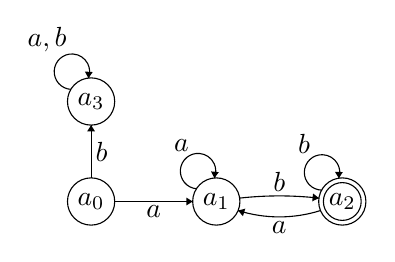
\begin{tikzpicture}[scale=0.10]
        \tikzstyle{every node}+=[inner sep=0pt]
        \draw [black] (15.9,-29.8) circle (3);
        \draw (15.9,-29.8) node {$a_0$};
        \draw [black] (15.9,-17.1) circle (3);
        \draw (15.9,-17.1) node {$a_3$};
        \draw [black] (31.8,-29.8) circle (3);
        \draw (31.8,-29.8) node {$a_1$};
        \draw [black] (47.8,-29.8) circle (3);
        \draw (47.8,-29.8) node {$a_2$};
        \draw [black] (47.8,-29.8) circle (2.4);
        \draw [black] (15.9,-26.8) -- (15.9,-20.1);
        \fill [black] (15.9,-20.1) -- (15.4,-20.9) -- (16.4,-20.9);
        \draw (16.4,-23.45) node [right] {$b$};
        \draw [black] (13.338,-15.561) arc (266.73523:-21.26477:2.25);
        \draw (10.31,-10.92) node [above] {$a,b$};
        \fill [black] (15.56,-14.13) -- (16.11,-13.36) -- (15.11,-13.3);
        \draw [black] (29.287,-28.183) arc (264.96376:-23.03624:2.25);
        \draw (27.38,-23.51) node [above] {$a$};
        \fill [black] (31.56,-26.82) -- (32.12,-26.07) -- (31.13,-25.98);
        \draw [black] (18.9,-29.8) -- (28.8,-29.8);
        \fill [black] (28.8,-29.8) -- (28,-29.3) -- (28,-30.3);
        \draw (23.85,-30.3) node [below] {$a$};
        \draw [black] (34.768,-29.369) arc (96.36866:83.63134:45.361);
        \fill [black] (44.83,-29.37) -- (44.09,-28.78) -- (43.98,-29.78);
        \draw (39.8,-28.59) node [above] {$b$};
        \draw [black] (45.184,-28.355) arc (268.82449:-19.17551:2.25);
        \draw (42.94,-23.76) node [above] {$b$};
        \fill [black] (47.36,-26.84) -- (47.87,-26.06) -- (46.87,-26.03);
        \draw [black] (45.032,-30.948) arc (-72.42971:-107.57029:17.333);
        \fill [black] (34.57,-30.95) -- (35.18,-31.67) -- (35.48,-30.71);
        \draw (39.8,-32.26) node [below] {$a$};
    \end{tikzpicture}
    \hspace{3em}
    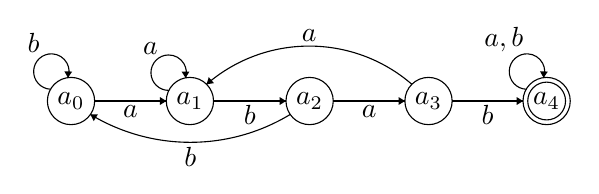
\begin{tikzpicture}[scale=0.10]
        \tikzstyle{every node}+=[inner sep=0pt]
        \draw [black] (7.4,-32.1) circle (3);
        \draw (7.4,-32.1) node {$a_0$};
        \draw [black] (22.5,-32.1) circle (3);
        \draw (22.5,-32.1) node {$a_1$};
        \draw [black] (37.7,-32.1) circle (3);
        \draw (37.7,-32.1) node {$a_2$};
        \draw [black] (52.8,-32.1) circle (3);
        \draw (52.8,-32.1) node {$a_3$};
        \draw [black] (67.8,-32.1) circle (3);
        \draw (67.8,-32.1) node {$a_4$};
        \draw [black] (67.8,-32.1) circle (2.4);
        \draw [black] (4.813,-30.604) arc (267.69007:-20.30993:2.25);
        \draw (2.65,-25.98) node [above] {$b$};
        \fill [black] (7.01,-29.14) -- (7.55,-28.36) -- (6.55,-28.32);
        \draw [black] (10.4,-32.1) -- (19.5,-32.1);
        \fill [black] (19.5,-32.1) -- (18.7,-31.6) -- (18.7,-32.6);
        \draw (14.95,-32.6) node [below] {$a$};
        \draw [black] (19.834,-30.75) arc (270.8699:-17.1301:2.25);
        \draw (17.5,-26.2) node [above] {$a$};
        \fill [black] (21.95,-29.16) -- (22.44,-28.36) -- (21.44,-28.37);
        \draw [black] (25.5,-32.1) -- (34.7,-32.1);
        \fill [black] (34.7,-32.1) -- (33.9,-31.6) -- (33.9,-32.6);
        \draw (30.1,-32.6) node [below] {$b$};
        \draw [black] (35.235,-33.806) arc (-58.8212:-121.1788:24.502);
        \fill [black] (9.87,-33.81) -- (10.29,-34.65) -- (10.81,-33.79);
        \draw (22.55,-37.85) node [below] {$b$};
        \draw [black] (40.7,-32.1) -- (49.8,-32.1);
        \fill [black] (49.8,-32.1) -- (49,-31.6) -- (49,-32.6);
        \draw (45.25,-32.6) node [below] {$a$};
        \draw [black] (55.8,-32.1) -- (64.8,-32.1);
        \fill [black] (64.8,-32.1) -- (64,-31.6) -- (64,-32.6);
        \draw (60.3,-32.6) node [below] {$b$};
        \draw [black] (24.614,-29.975) arc (130.83672:49.16328:19.936);
        \fill [black] (24.61,-29.98) -- (25.55,-29.83) -- (24.89,-29.07);
        \draw (37.65,-24.62) node [above] {$a$};
        \draw [black] (65.213,-30.604) arc (267.69007:-20.30993:2.25);
        \draw (62.36,-25.98) node [above] {$a,b$};
        \fill [black] (67.41,-29.14) -- (67.95,-28.36) -- (66.95,-28.32);
    \end{tikzpicture}
    \label{fig:fin_state_mach}
    \caption{The finite state machines for all strings starting in `a' and ending in `b' (left) and all strings containing `abab'.}
\end{figure}

\section{Context-free grammar}

Just as we use regular expressions in lexical analysis, we can use a \textbf{context-free grammar} to describe the syntax of a programming language. Our primary goal here is to take a token stream and decide whether it corresponids to a legitmate program or not, so that if it does then we can proceed with compilation.

\begin{definition}[Formal grammar]
    In formal language theory, a \textbf{grammar} (or \textbf{formal grammar}), is a set of production rules for strings in a formal language. The rules describe how to form strings from the language's alphabet that are valida ccording to the language's syntax.
\end{definition}

\begin{definition}[Context-free grammar]
    A context-free grammar $G$ is a type of formal grammar where production rules are limited to simple replacements. $G$ is defined by the 4-tuple $G = (V, \Sigma, R, S)$ where 
    \begin{enumerate}
        \item $V$ is a finite set of nonterminal characters called \textbf{variables}, note that $V \subset G$;
        \item $\Sigma$ is a finite set of \textbf{terminals}, disjoint from $V$;
        \item $R$ is a finite relation from $V$ to $(V \cup \Sigma)^\star$ (where $\star$ represents the Kleene star operation from before) called the \textbf{rules} of the grammar; and
        \item $S \in V$ is the start variable, used to represent the whole sentence.
    \end{enumerate}
    A production rule in $R$ is described as a pair $(\alpha, \beta) \in R$ where $\alpha \in V$ is a variable and $\beta \in (V \cup \Sigma)^\star$ is a string of variables and / or terminals. We typically use the notation $\alpha \to \beta$ for this.
\end{definition}

\begin{remark}
    For a context-free grammar $G = (V, \Sigma, R, S)$, with a production rule $(\alpha, \beta) \in R$, $\beta$ is allowed to be the empty string, denoted $\beta \to \varepsilon$. This is called $\varepsilon$-production. Additionally, if $\alpha \to \beta_1$ and $\alpha \to \beta_2$, it is typical to write $\alpha \to \beta_1 \mid \beta_2$. 
\end{remark}

Productions in context-free grammar are of the form \[ b \to a_1 a_2 \ldots a_n \] where $n \geq 0$, $b \in N$, and $a_1, \ldots, a_n \in N \cup T$.

\begin{example}
    Consider the context-free grammar \[ G = (V = \{ s, t, u \}, \Sigma = \{ a, b \},  R, s) \] where \[ \{ s \to \varepsilon, \; s \to bs, \; s \to at, \; t \to bs, \; t \to \varepsilon, \; t \to au \}. \] From this we derive $b^nabs$ for some $b \geq 0$.
\end{example}

\section{Syntax analysis}

\begin{definition}
    Programming language syntax is almost always describable by a \textbf{context-free grammar}. A \textbf{(phase-structure) grammar} is a tuple $(N,T,s,R)$ where
    \begin{enumerate}
        \item $T$ and $N$ are disjoint finite sets of terminal and non-terminal symbols, respectively.
        ;
        \item $s\in N$ is the start symbol; and
        \item $R$ is a finite set of productions or rules so that
        \[R\subset(N\cup T)^+\times(N\cup T)^*\]
        where if $(\alpha,\beta)\in R$ then $\alpha$ contains at least one symbol from $N$.
    \end{enumerate}
    In a context-free grammar, productions are of the form
    \[b\rightarrow a_1a_2\ldots a_k\]
    with $k\geq0,b\in N$ and $a_1,a_2,\ldots,a_k\in N\cup T$.
\end{definition}

\begin{definition}
    A \textbf{regular grammar} is a context-free grammar where all productions are of one of the following forms:
    \begin{enumerate}
        \item $b\rightarrow a$ where $a\in T$;
        \item $b\rightarrow ac$ where $a\in T,c\in N$; or
        \item $b\rightarrow c$.
    \end{enumerate}
\end{definition}

\begin{theorem}
    A set of strings is represented by a regular expression if, and only if, it is accepted by a finite state machine if, and only if, it s generated by some regular grammar.
\end{theorem}

% section this off properly and look at notes for examples and more description

\section{Backus Naur Form}

\begin{definition}
    Context-free grammars are usually expressed in Backus Naur Form (BNF):
    
    \begin{enumerate}
        \item productions with the same left-hand sides be separated with $|$ (so as to denote choice);
        \item non-terminals appear inside ; and
        \item $::=$ is used instead of $\rightarrow$.
    \end{enumerate}
\end{definition}
